%\documentclass[onecolumn]{IEEEtranTIE}
\documentclass[journal]{IEEEtranTIE}
\usepackage{graphicx}
\usepackage{cite}
\usepackage{picinpar}
\usepackage{amsmath}
\usepackage{url}
\usepackage{flushend}
\usepackage[latin1]{inputenc}
\usepackage{colortbl}
\usepackage{soul}
\usepackage{multirow}
\usepackage{pifont}
\usepackage{color}
\usepackage{alltt}
\usepackage[hidelinks]{hyperref}
\usepackage{enumerate}
\usepackage{siunitx}
\usepackage{breakurl}
\usepackage{epstopdf}
\usepackage{pbox}
\usepackage{float}
\usepackage{algorithm2e}
\usepackage{nomencl}

\makenomenclature
\SetKwComment{Comment}{/* }{ */}

\begin{document}
\title{	Preparation of Papers for IEEE}

\author{
	\vskip 1em
	
	First A. Author1, \emph{Student Membership},
	Second B. Author2, \emph{Membership},
	\\ and Third C. Author3, \emph{Membership}

	\thanks{
	
		Manuscript received Month xx, 2xxx; revised Month xx, xxxx; accepted Month x, xxxx.
		This work was supported in part by the xxx Department of xxx under Grant  (sponsor and financial support acknowledgment goes here).
		
		(Authors' names and affiliation) First A. Author1 and Second B. Author2 are with the xxx Department, University of xxx, City, Zip code, Country, on leave from the National Institute for xxx, City, Zip code, Country (e-mail: author@domain.com). 
		
		Third C. Author3 is with the National Institute of xxx, City, Zip code, Country (corresponding author to provide phone: xxx-xxx-xxxx; fax: xxx-xxx-xxxx; e-mail: author@ domain.gov).
	}
}

\maketitle

\begin{abstract}
These instructions give you guidelines for preparing papers for IEEE TRANSACTIONS ON INDUSTRIAL ELECTRONICS. 
Use this document as a template. The electronic file of your paper will be formatted further at IEEE. Paper titles should be written in uppercase and lowercase letters, not all uppercase. Avoid writing long formulas with subscripts in the title; short formulas that identify the elements are fine (e.g., ``Nd-Fe-B''). Do not write ``(Invited)'' in the title. Write full names of authors in the author field. Define all symbols used in the abstract. Do not cite references in the abstract. Do not delete the blank line immediately above the abstract; it sets the footnote at the bottom of this column.
sdfhlkashdflkasdhfklasdf
\end{abstract}

\begin{IEEEkeywords}
    Enter key words or phrases in alphabetical order, separated by commas. For a list of suggested keywords, send a blank e-mail to \href{mailto:keywords@ieee.org}{keywords@ieee.org} or visit \url{http://www.ieee.org/documents/taxonomy_v101.pdf}.
    \end{IEEEkeywords}

    \markboth{IEEE TRANSACTIONS ON INDUSTRIAL ELECTRONICS}%
    {}
    
    \definecolor{limegreen}{rgb}{0.2, 0.8, 0.2}
    \definecolor{forestgreen}{rgb}{0.13, 0.55, 0.13}
    \definecolor{greenhtml}{rgb}{0.0, 0.5, 0.0}
\nomenclature{$\eta$}{energy outflow curve}
\nomenclature{$\mathcal{U}_t$}{uncertainty set for $Q_{in,t}$ at time $t$}
\nomenclature{$\sigma_t$}{Slack variable at time $t$}
\nomenclature{$\ell$}{number of lags}
\nomenclature{$\Lambda_t$}{Regularization Vector}
\nomenclature{$H$}{Upper MPC horizon}
\nomenclature{$h$}{Lower MPC horizon}
\nomenclature{$h$}{Tank's height}
\nomenclature{$h_{ref}$}{Height Reference}
\nomenclature{$E$}{Energy Consuption}
\nomenclature{$Q_{out}$}{Hourly Outflow of the Tank}
\nomenclature{$\pi$}{Day-ahead energy price}
\nomenclature{$\hat{Q}_{in}$}{Forecasted Inflow per hour}
\nomenclature{$\omega_j$}{j-th Pump speed}
\nomenclature{$q_{out,j}$}{Outflow of the j-th pump }
\nomenclature{$q_{in}$}{Estimate of the inflow per minute.}
\nomenclature{$p_{j}$}{Pipe-line Pressure}
\printnomenclature


% run the nomenclature after finishing this

%makeindex paper.nlo -s nomencl.ist -o paper.nls


\section{Introduction}

\IEEEPARstart{P}{ower} electronic converters (PECs) are ubiquitous, serving as critical interfaces in electrification by connecting loads, energy storage systems, sources, and the grid. For example, PECs are used to convert alternating current (AC) to direct current (DC) in electric vehicles (EVs), transform DC to AC in photovoltaic systems to align with grid frequency and voltage and facilitate operations in high-power applications and various industrial processes, mainly electric drives. 
As Europe progresses in its green transition and electrification actions, 
it becomes clear how PECs have a major role in orchestrating 
a large network of \textit{prosumers}, i.e., flexible loads that could serve as consumers or producers based on the operational
grids. Today, most industrial applications are still unidirectional, meaning they consume energy according to their strategy without taking grid conditions into account, primarily due to the fact that energy generation was traditionally dominated by large plants operating on a fixed schedule to meet specific demands during designated hours.
However, in addition to the inverter-based grid, and stability challenges,
with the energy landscape gradually shifting from centralized to decentralized and stochastic generation, it also pushes for significant technological advancements. 


However, the aggregation of this flexibilities come with a price,
especially in terms of data aggregation, computational resources, scalability and advances control 
techniques that are able to interact with cloud architecture, PLCs and APIs. (Read paper Musumeci) 


Small summaries of paper analyzing could platform with gree transitions


\cite{bagherzadeh2020integration} analyzes the challanges in communication, storages and computational capabilities in 
massive streams of data, while \cite{shahinzadeh2018green} presents how IoT benefit the accurate forecasting and predictive mantainance ensuring high security levels. 
Paper \cite{hossein2020internet} extensively review the literature on the application of IoT in energy sectors ans smart grids, by 
distinguishes the the transmission and distribution levels, where IoT can be applied to energy efficiency, aggregation of distributed generations and electric vehicles
aggregation (V2G), from the demand side where IoT can be used for battery energy storage management and control to smart building control. 

Wi-Fi, Bluetooth, ZigBee \cite{karunarathne2018wireless} LTE-4G and 5G networks \cite{li20185g}



As an example in paper 1 the authors studies the return of investment of the design
of distributed energy resources. Other studies focuses on how a distributed scenario could benefit the industry, 
or how policy maker could push for emerging markets for distribute resources. On the bottom level, the integration of grid-based inverters
playing a pivotal role in designing a grid able to maintain a power quality and stability.
In fact it is known that with the increasing amount of renewables, the grid is being more exposed to fluctation 
and stochasticty mainly driven by the weather forecast, requiring the energy storage and ancillary service includes 
managing voltage levels and frequency to prevent grid disturbances.
Another part of the literature is focusing on scheduling and resource allocation under uncertainty. 
Methods like stochastic or robust optimization are now becoming more popular in order to minimize Value at Risk (VAr), under uncertain conditions. 

\section{System Description}
The cloud is a service where all the application can be executed on a virtual 
environment owned either by privite or company. In our application, we used the 
Internet of Things (IoT) Hub from Azure, which is a centralized platform that facilitates the 
connections and the management of fleets of IoT devices. The IoT Hub enables a streamlined 
bidirectional comunication from the Cloud to the physical devices, sensors.
As reported above, nowadays most of the energy plant are equipped with SCADA 
(Supervisory Control and Data Acquisition) \cite{daneels1999scada}, which enables data 
real-time monitoring and control of industrial processes and infrastructure.
It integrates hardware and 
software components to collect data from sensors, control equipment, and provide 
centralized oversight through Human-Machine Interfaces (HMIs). However, in comparison with SCADA, the IoT Hub has some more 7
support in terms of scalability, as it can support thousand of sensors and embedded devices, and also provide an extra layer of 
flexibility in terms of data collection for real-time and historical data. Moreover, it also provides different technologies for 
data driven modelling and artificial intelligence services. 

IoT sensors can be controlled singularly from the Azure Hub, but this is not our case. In our application, all the sensors are 
aggregated using a Kunbus Revolution Pi, which is the industrial standard of Revolution Pi. 
The Revolution Pi enables a bi-directional communication and serves as bridge between the PLC and the Cloud. 
The communication between the Gateway and the PLC is Modbus TCP/IP, a tailored version of the protocol for network communication 
over internet. One of the key advantage of this chain strategy is that the majority of the sensors, VDFs are connected to the 
PLC directly, so there is not need to rebuild from scratch the communication between all the sensor and the RevPi. 
The PLC is the Siemens s7-1200, which support Profinet, a propetary version of Profibus protocol, developed by Siemens that enable fast and reliable communication in control. 
The PLC is the connected to the following devices: VDF1, VDF2, VDF3, Outflow sensor, level sensor, pressure sensor, 
Addionally, from each VDF can be retrieved the instantaneous speed and power consumption. 

A crucial role in this application is played by the RevPi which not only combine the collected data from the 
PLC and the gateway and pushes the data to the cloud but also acts as real-time controller, overcoming the limitation 
of the PLC in terms of computational capabilities. In fact, the needs more comprehensive and optimization based control techniques 
, poses the needs of extra computational power, memory allocation and faster CPUs.
This architecture, compared to purely cloud-based controller, provides an extra layer of security, as the the on-site control device, can able to handle different 
situations, overcoming well-known limitations broader adoption, as delays or disruptions in communications.


\begin{figure*}[h]
    \centering
    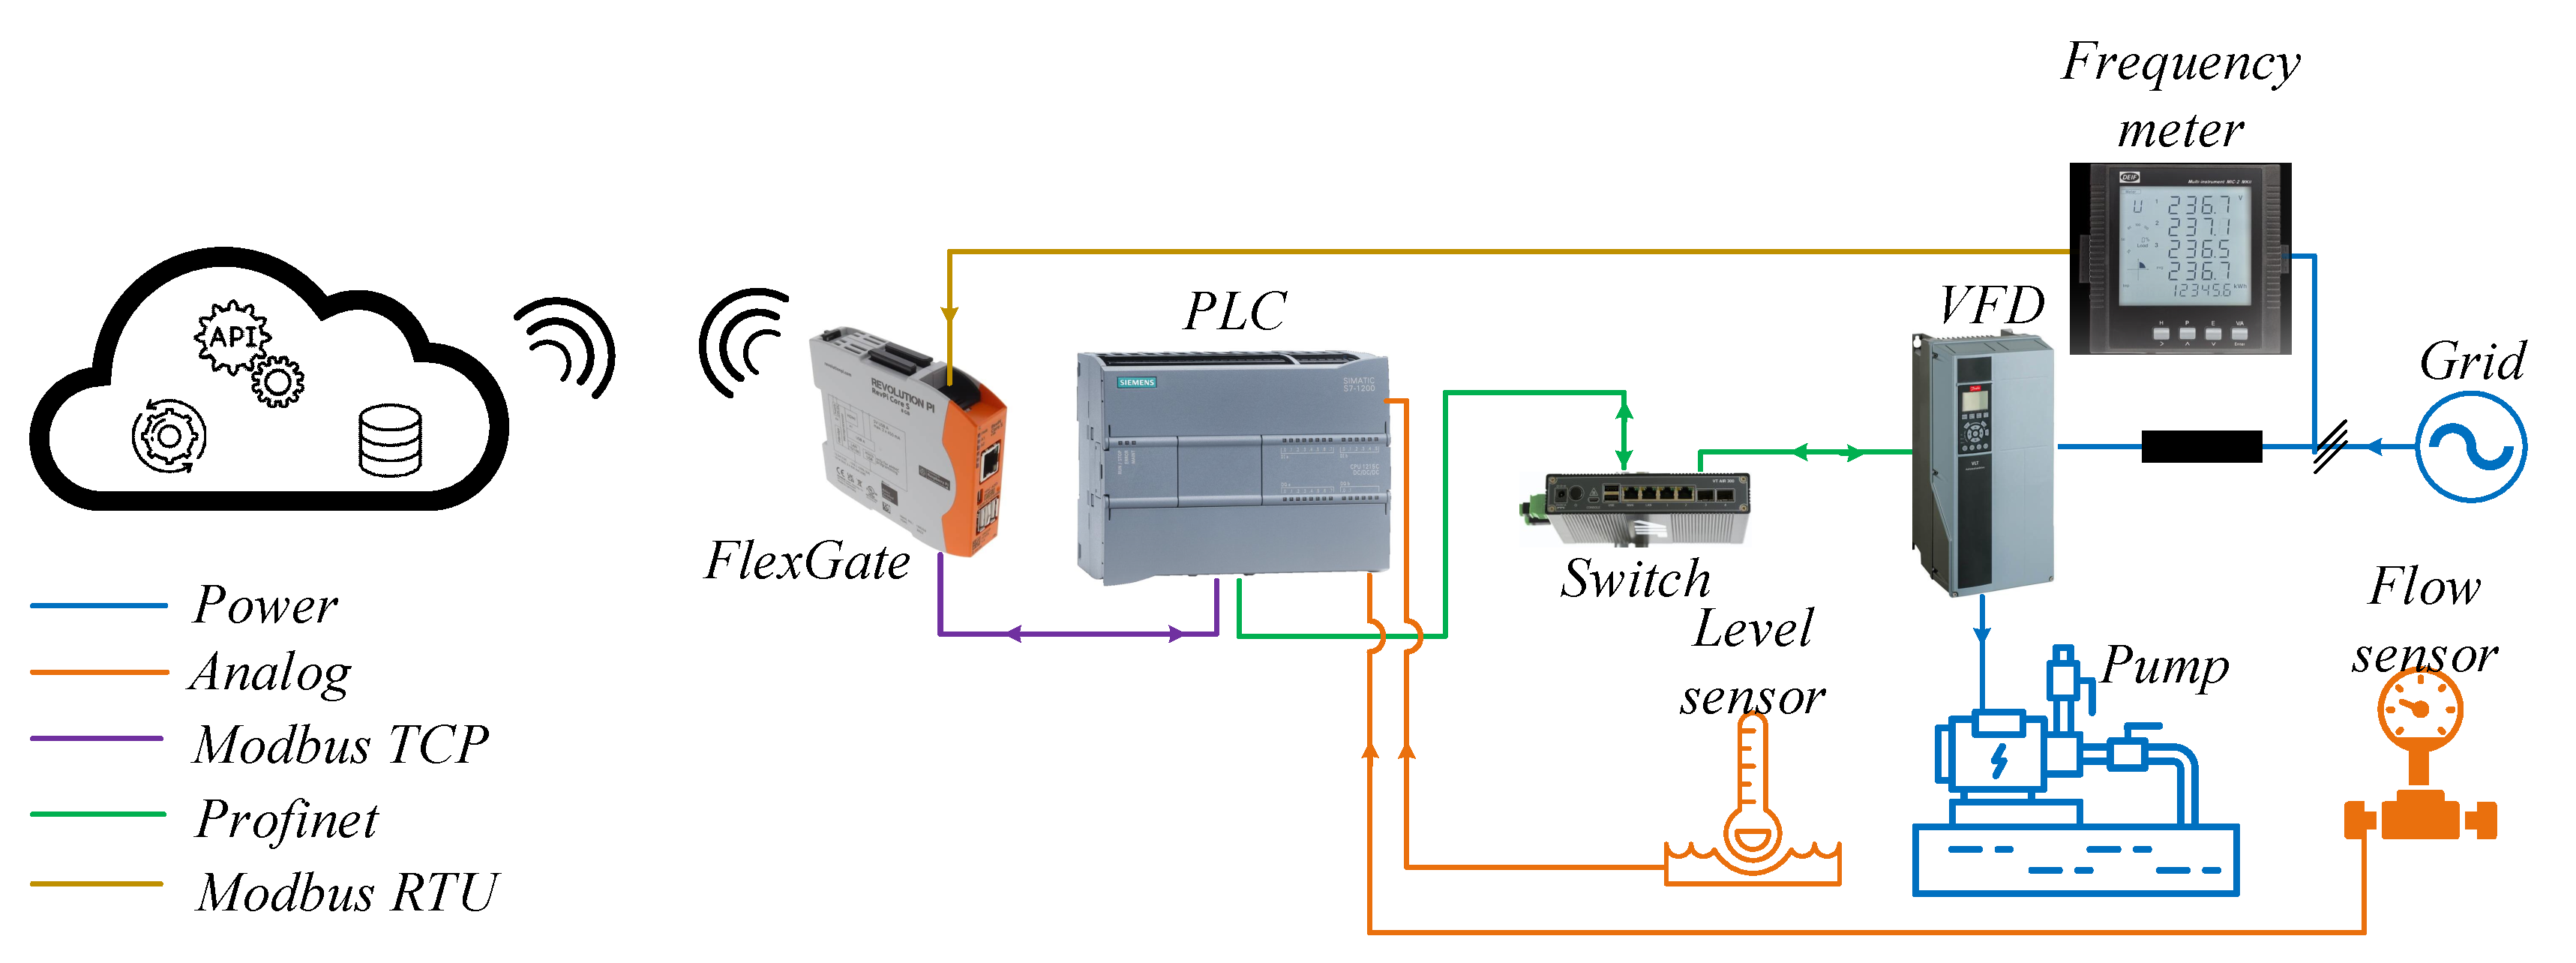
\includegraphics[width=0.8\textwidth]{img/test.pdf}
    \caption{Your caption text.}
    \label{fig:your_label}
\end{figure*}


\subsubsection{Data streaming and Features.}
The resolution frequency of the data streaming is $1\si{\hertz}$, as every second one measurement is sampled, pushed and stored to a time series database 
located in the cloud. Each sensor has a time index and values and can be queried from external APIs. 
This architecture allows high modularity as different blocks perform different operation




\begin{table}[!t]
    \renewcommand{\arraystretch}{1.3}
    \caption{Units for Magnetic Properties}
    \centering
    \label{table_1}
    \resizebox{0.8\columnwidth}{!}{
        \begin{tabular}{c c c}
            \hline\hline \\[-3mm]
            \multicolumn{1}{c}{Sensor} & \multicolumn{1}{c}{Unit of Measurement} & \multicolumn{1}{c}{Protocol} \\[1.6ex] \hline
            $ \rm{Level} $  & \si{\meter} & \textit{Analog} \\
            $ \rm{Speed} $ & \si{rpm} & \textit{Profinet} \\ 
            $ \rm{Inflow} $ & \si{\meter^3}/\si{\hour} & \textit{Virtual} \\ 
            $ \rm{Power} $ & \si{kW}/\si{\hour} & \textit{Profinet} \\ 

            $ \rm{Pressure} $  & \si{psi} & \textit{Profinet} \\
            $ \rm{Outflow} $ & \si{\meter^3}/\si{\hour} & \textit{Analog} \\ 

            \hline\hline
        \end{tabular}
    }
\end{table}


\begin{figure}[H]
    \centering
    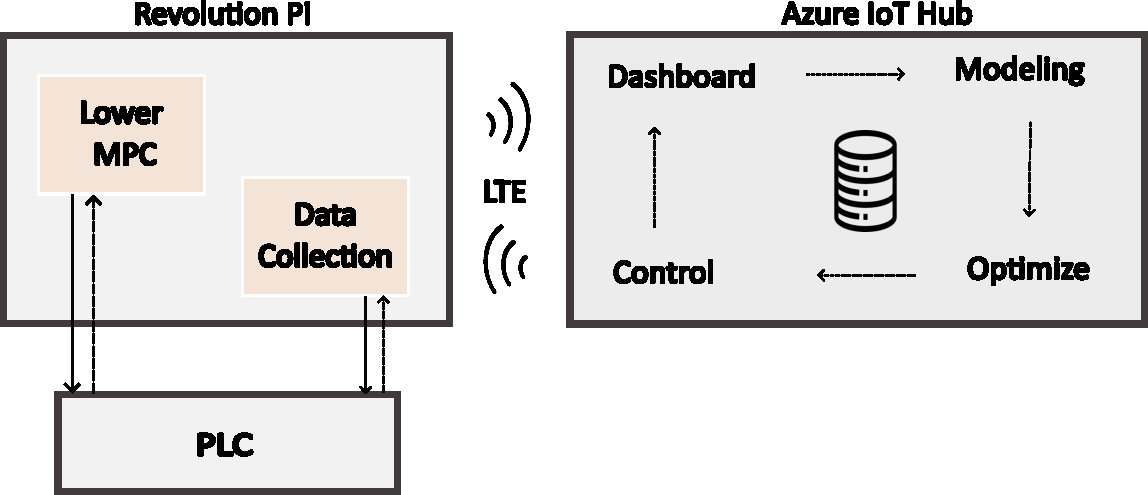
\includegraphics[width=0.45\textwidth]{img/block_diagram.pdf}
    \caption{Edge-Cloud Architecture }
    \label{fig:your_label}
\end{figure}






\section{System Description}

The cloud is a service where all the application can be executed on a virtual 
environment owned either by private or company. In our application, we used the 
Internet of Things (IoT) Hub from Azure, which is a centralized platform that facilitates the 
connections and the management of fleets of IoT devices. The IoT Hub enables a streamlined 
bidirectional comunication from the Cloud to the physical devices, sensors.
As reported above, nowadays most of the energy plant are equipped with SCADA 
(Supervisory Control and Data Acquisition) \cite{daneels1999scada}, which enables data 
real-time monitoring and control of industrial processes and infrastructure.
It integrates hardware and 
software components to collect data from sensors, control equipment, and provide 
centralized oversight through Human-Machine Interfaces (HMIs). However, in comparison with SCADA, the IoT Hub has some more 7
support in terms of scalability, as it can support thousand of sensors and embedded devices, and also provide an extra layer of 
flexibility in terms of data collection for real-time and historical data. Moreover, it also provides different technologies for 
data driven modelling and artificial intelligence services. 

IoT sensors can be controlled singularly from the Azure Hub, but this is not our case. In our application, all the sensors are 
aggregated using a Kunbus Revolution Pi, which is the industrial standard of Revolution Pi. 
The Revolution Pi enables a bi-directional communication and serves as bridge between the PLC and the Cloud. 
The communication between the Gateway and the PLC is Modbus TCP/IP, a tailored version of the protocol for network communication 
over internet. One of the key advantage of this chain strategy is that the majority of the sensors, VDFs are connected to the 
PLC directly, so there is not need to rebuild from scratch the communication between all the sensor and the RevPi. 
The PLC is the Siemens s7-1200, which support Profinet, a propetary version of Profibus protocol, developed by Siemens that enable fast and reliable communication in control. 
The PLC is the connected to the following devices: VDF1, VDF2, VDF3, Outflow sensor, level sensor, pressure sensor, 
Addionally, from each VDF can be retrieved the instantaneous speed and power consumption. 

A crucial role in this application is played by the RevPi which not only combine the collected data from the 
PLC and the gateway and pushes the data to the cloud but also acts as real-time controller, overcoming the limitation 
of the PLC in terms of computational capabilities. In fact, the needs more comprehensive and optimization based control techniques 
, poses the needs of extra computational power, memory allocation and faster CPUs.
This architecture, compared to purely cloud-based controller, provides an extra layer of security, as the the on-site control device, can able to handle different 
situations, overcoming well-known limitations broader adoption, as delays or disruptions in communications.


\begin{figure}[h]
    \centering
    \hspace{2cm}
    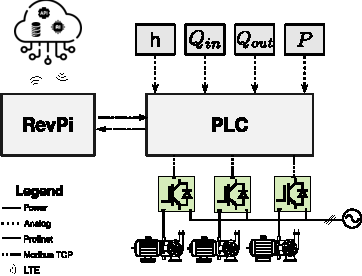
\includegraphics[width=0.5\textwidth]{img/schematic.pdf}
    \caption{Your caption text.}
    \label{fig:your_label}
\end{figure}


\subsubsection{Data streaming and Features.}
The resolution frequency of the data streaming is $1\si{\hertz}$, as every second one measurement is sampled, pushed and stored to a time series database 
located in the cloud. Each sensor has a time index and values and can be queried from external APIs. 
This architecture allows high modularity as different blocks perform different operation



\begin{table}[!t]
    \renewcommand{\arraystretch}{1.3}
    \caption{Sensors Overview}
    \centering
    \label{table_1}
    \resizebox{0.8\columnwidth}{!}{
        \begin{tabular}{c c c}
            \hline\hline \\[-3mm]
            \multicolumn{1}{c}{Sensor} & \multicolumn{1}{c}{Unit of Measurement} & \multicolumn{1}{c}{Protocol} \\[1.6ex] \hline
            $ \rm{Level} $  & \si{\meter} & \textit{Analog} \\
            $ \rm{Speed} $ & \si{rpm} & \textit{Profinet} \\ 
            $ \rm{Inflow} $ & \si{\meter^3}/\si{\hour} & \textit{Virtual} \\ 
            $ \rm{Power} $ & \si{kW}/\si{\hour} & \textit{Profinet} \\ 

            $ \rm{Pressure} $  & \si{psi} & \textit{Profinet} \\
            $ \rm{Outflow} $ & \si{\meter^3}/\si{\hour} & \textit{Analog} \\ 

            \hline\hline
        \end{tabular}
    }
\end{table}


\begin{figure}[H]
    \centering
    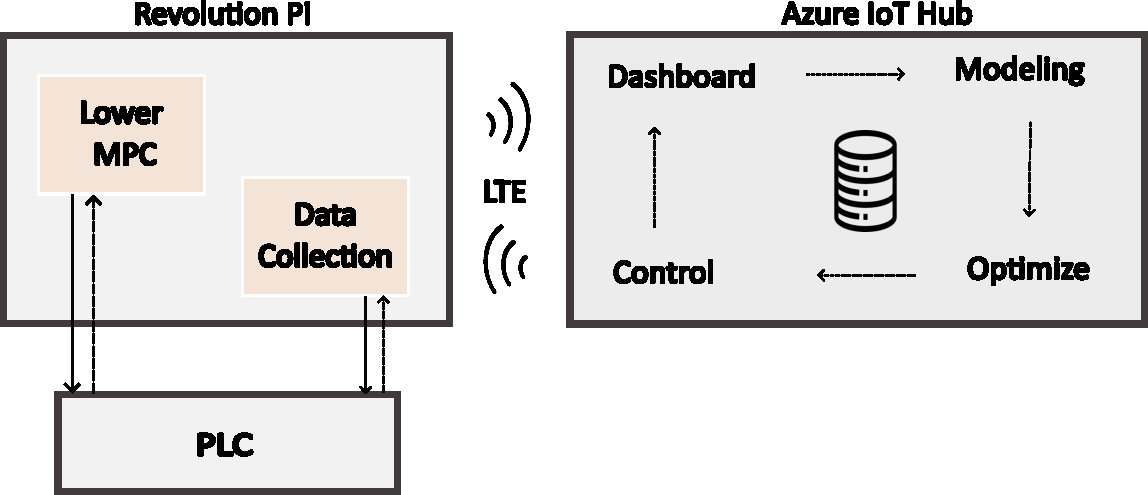
\includegraphics[width=0.49\textwidth]{img/block_diagram.pdf}
    \caption{Edge-Cloud Architecture }
    \label{fig:your_label}
\end{figure}
\section{System Identification}
\subsection{ARX Model}
	We have chosen to represent the system in \textit{discrete time},
	\begin{align}
		y_t &+ a_1 y_{t-1} + \cdots + a_n y_{t-p} = b_1 u_{t-1} + \cdots + b_q u_{t-q}
	\end{align}

	\begin{align}
		\theta = \begin{bmatrix}
		a_1, \ldots, a_p, b_1, \ldots, b_q
		\end{bmatrix}^T
	\end{align} 

	\begin{align}
		\varphi(t) = \begin{bmatrix}
		-y_{t-1} \cdots - y_{t-p}, u_{t-1} \cdots u_{t-q}
		\end{bmatrix}^T
	\end{align}

	\begin{align}
		y_t = \varphi^T_t \theta_t \quad  \forall t \in (1, N)
	\end{align}



	For a given system we can collect inputs and outputs over a time
	interval $t$

	\begin{align}
		\emph{Z}^N = \big \{u(t_0), y(t_0), \cdots, u(N), y(n)\big \}
	\end{align}


	\begin{align}
		\hat{\theta} = \arg\min_{x} \emph{V}_N(\theta) + \lambda(\theta - \theta^*)R(\theta - \theta^*)
	\end{align}

	The ARX(p, q) model is given by:
	\begin{align}
	y_t = \sum_{i=1}^p \varphi_i y_{t-i} + \sum_{j=1}^q \beta_j x_{t-j} + \epsilon_t
	\end{align}


\subsection{Piecewise Linear function}

	\begin{algorithm}
		\caption{Grouping Time Series Data by Bin Medians}
		\begin{algorithmic}[1]
		\REQUIRE Time series data \( y = \{y_1, y_2, \ldots, y_T\} \), excitation data \( u = \{u_1, u_2, \ldots, u_T\} \), bin size \( n \)
		\ENSURE Grouped data by bin medians
		
		\STATE Divide the time series \( y \) into bins of size \( n \)
		\FOR{$i = 1$ to $\left\lceil \frac{T}{n} \right\rceil$}
			\STATE $B_i \gets \{ y_{(i-1)n+1}, y_{(i-1)n+2}, \ldots, y_{\min(in, T)} \}$
			\STATE Compute the median \( m_i \) of the bin \( B_i \)
		\ENDFOR
		
		\STATE Group the data in \( y \) by their corresponding bin medians \( m_i \)
		
		\end{algorithmic}
		\end{algorithm}


\section{Inflow Estimation}

	The considered wastewater pumping station, only the outflow and the height are measured, 
	while the inflow is not measured or estimated. Therefore, in order to estimate the inflow of the tank, 
	we implemented an observer by using the tank equation where the instantaneous rate of change of the height $dh$ is proportional 
	to the difference between the inflow and the outflow of the tank, scaled by the area of the tank, as pointed Eq.\ref{eq:height_eq}.
	\begin{align}
	h_t = h_0 + \frac{T_s}{A}(Q_{in,t} - Q_{out,t}) + v_t \label{eq:height_eq}
	\end{align}

	\noindent where \( A \), the cross-sectional area of the tank, $T_s$ is the sampling time of the measurements,
	$Q_{in,t}$ and $Q_{out,t}$ are the measured inflow and outflow respectively, and $v_t$ is the measurement noise. 

	By defining the the inflow  \( Q_{in,t} \) any time \( t \), the hidden state the 
	Eq.\ref{eq:height_eq}, \( w_t \) the process noise, \( Q \) is the covariance of the process noise, and \( R \) is the measurement noise covariance.
	\[
	Q_{in, t+1} = Q_{in, t} + w_t
	\]
	
	\noindent The states can be estimated by means of the Kalman filter, at any given time \( t \)
	\subsubsection*{Prediction Step}
	\begin{align*}
	\hat{Q}_{in, t+1|t} &= \hat{Q}_{in,t|t} \\
	P_{t+1|t} &= P_{t|t} + Q
	\end{align*}
	where \( Q \) is the covariance of the process noise.

	\subsubsection*{Update Step}
	Compute the Kalman Gain and update the estimate with the measurement:

	\begin{align*}
		\Delta h_{t+1} &= h_{t+1} - z_{h,t+1} \\
		\Delta Q_{t+1} &= \hat{Q}_{in,t+1|t} - z_{Q_{out},t+1} \\
		\hat{Q}_{in,t+1|t+1} &= \hat{Q}_{in,t+1|t} + K_{t+1} \left(\frac{A}{T_s}\Delta h_{t+1} - \Delta Q_{t+1} \right)
		\end{align*}
	
\


\section{Inflow Forecast}

\section{Hierarchical Model Predictive Control}
	\subsection{Higher-Level MPC}
		\begin{subequations}\label{P0:higher_mpc}
			\begin{align}
				\underset{\zeta, }{\text{min}}& \sum_{t=1}^{T} \Gamma \left\lVert E \right\rVert^{2}_{t} + \Lambda_t^T \sigma_t   \label{P0:1} \\
				&\hspace{-1em} \text{s.t.}  \quad \quad \forall \sigma_t \geq 0 \label{P0:2} \\
				& \qquad \zeta_{t} = \sum_{j=1}^3 \zeta_{t-1} \label{P0:3}  \\
				& \qquad Q_{in,t} \leq 0\label{P0:4} \\
				& \qquad h_{min}\leq h_{t} \leq h_{max}\label{P0:5}\\
				& \qquad E_{min}\leq E_{t} \leq E_{max}\label{P0:6}
		\end{align}
		\end{subequations}
	

\subsection{Lower-Level MPC}
	\begin{subequations}\label{P2:FinalModel}
		\begin{align}
			\underset{\omega, E, P, Q_{\text{out}}}{\text{min}}& \sum_{k=1}^{h} \mathcal{Q} \left\lVert h_k - h_r \right\rVert^2 + \mathcal{R} \left\lVert \omega_k \right\rVert^2 + \Gamma \left\lVert E \right\rVert^{2}_{k} + \Lambda_k^T \sigma_k  \label{P1:lower_mpc} \\
			&\hspace{-1em} \text{s.t.}  \quad \quad \forall \sigma_k \geq 0, \; l \geq 0 \label{P1:1} \\
			& \qquad Q_{\text{out}, k} = \sum_{j=1}^3 Q_{out_{j,k-1}} \label{P1:2} \\
			& \qquad E_{k} = \sum_{j=1}^3 E_{k-l} \label{P1:3}  \\
			& \qquad P_{k} = \sum_{j=1}^3 P_{k-l} \label{P1:4}  \\
			& \qquad Q_{in,k} = \tilde{Q}_{in,k-1} \label{P1:5}  \\
			& \qquad h_k = \frac{1}{A} \Big(\tilde{Q}_{in,k} - Q_{out,k}\Big) \label{P1:6} \\
			& \qquad \omega_{l} - \sigma_{\omega} \leq \omega_k \leq \omega_{u} + \sigma_{\omega} \label{P1:7} \\
			& \qquad P_{l} - \sigma_{P} \leq P_k \leq P_{u} + \sigma_{P} \label{P1:8} \\
			& \qquad h_{r} - \sigma_{h_{r}} \leq h_k \leq h_{l} + \sigma_{h_{r}} \label{P1:9}
	\end{align}
	\end{subequations}
\section{Experimental Results}
\section{Conclusion}
\bibliographystyle{bibliography/IEEEtranTIE}
\bibliography{bibliography/IEEEabrv,bibliography/BIB_xx-TIE-xxxx}\ %IEEEabrv instead of IEEEfull

\end{document}
